\begin{figure}[htbp]
    \begin{center}
        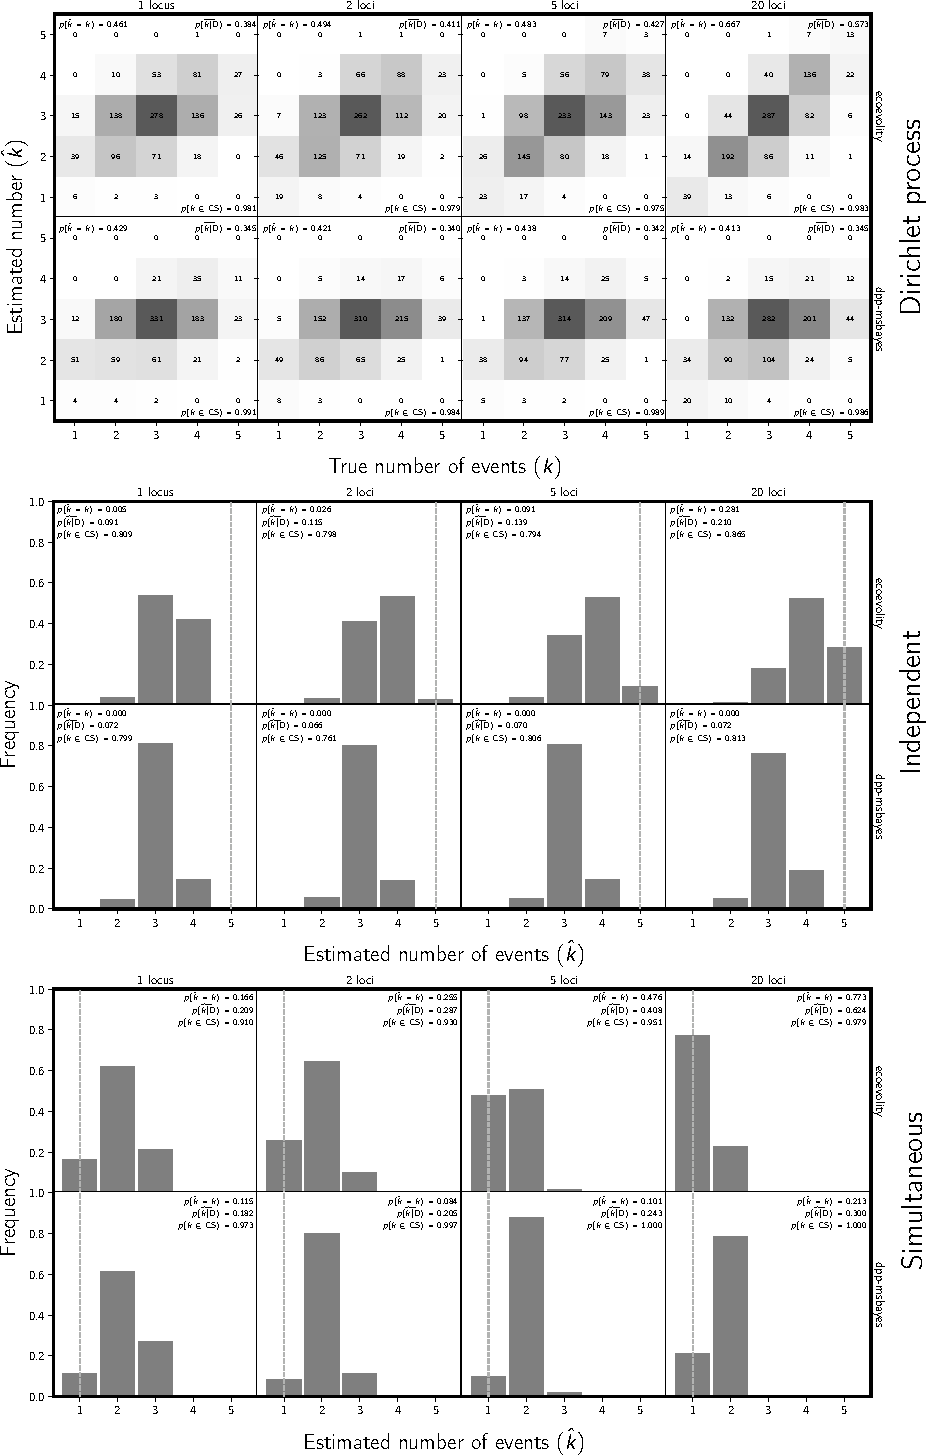
\includegraphics[width=\textwidth,height=0.9\textheight,keepaspectratio]{../images/from-project-repo/plots/tex-plot-grids/grid-nevents-cropped.pdf}
        \caption{
            \scriptsize
            \Ecoevolity better estimates the number of divergence
            events than \dppmsbayes across all simulated numbers of
            loci (columns) for five pairs of populations simulated to have
            diverged according to a Dirichlet process (top 8 plots),
            indepedently (middle 8 plots),
            or
            simultaneously (bottom 8 plots).
            \neventsshadingdescription{}
            \neventsplotannotations{}
        }
        \label{fig:nevents}
    \end{center}
\end{figure}

\clearpage

\begin{figure}[htbp]
    \begin{center}
        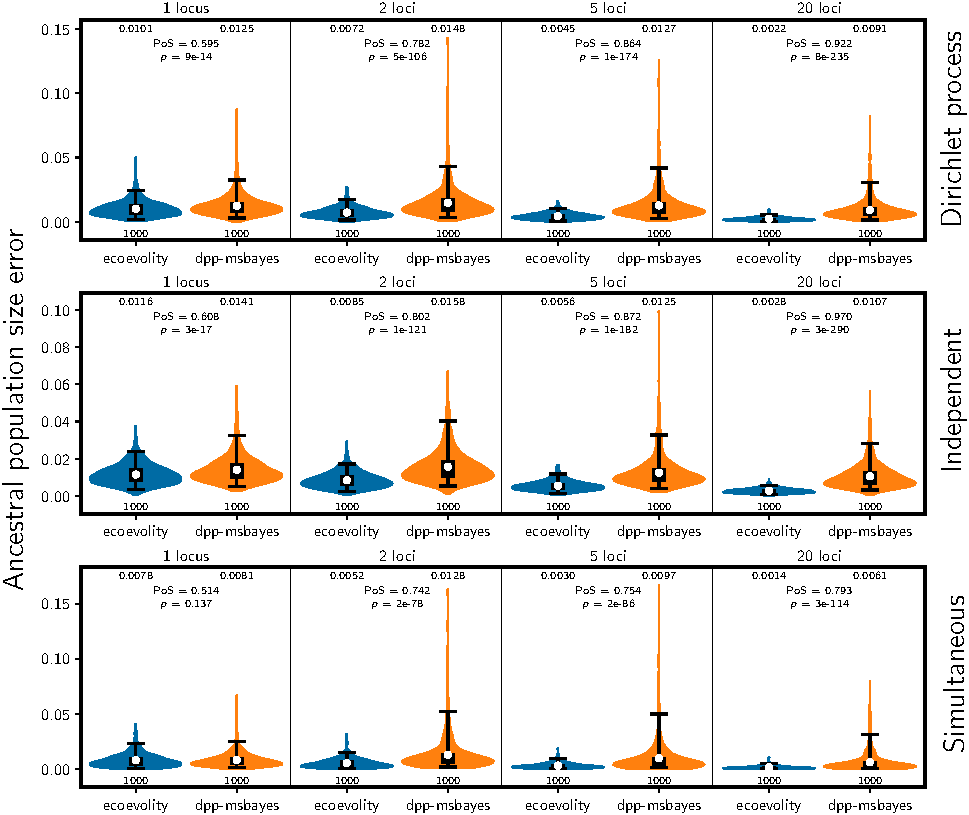
\includegraphics[width=\textwidth,height=\textheight,keepaspectratio]{../images/from-project-repo/plots/tex-plot-grids/grid-ancestral-pop-size-error-cropped.pdf}
        \caption{
            \scriptsize
            \Ecoevolity better estimates the effective size of the ancestral
            populations than \dppmsbayes across all simulated numbers of loci
            (columns) and whether the divergence model was drawn from a
            Dirichlet process (top row), or constrained so that all pairs of
            populations diverged independently (middle row) or simultaneously
            (bottom row).
            Error was quantified for each simulation replicate
            as the sum of the difference between the true and posterior mean
            population size across the five pairs of populations.
            For each violin plot, the sample size (number of simulation
            replicates) is shown beneath and the mean is represented by the
            white dot and shown above.
            The box shows the upper and lower quartiles and the brackets
            show the 2.5th and 97.5th percentiles.
            At the top center of each plot, the results of a Mann-Whitney U
            test \citep{MannWhitney1947} are shown comparing mean model errors
            between \ecoevolity and \dppmsbayes;
            the probability of superiority \citep[PoS, the probability that
            \ecoevolity has a lower mean model error than \dppmsbayes for a
            random simulation replicate drawn from
            each;][]{WolfeHogg1971,Grissom1994} and p-value is provided.
        }
        \label{fig:ancpopsizeerror}
    \end{center}
\end{figure}

\clearpage

\begin{figure}[htbp]
    \begin{center}
        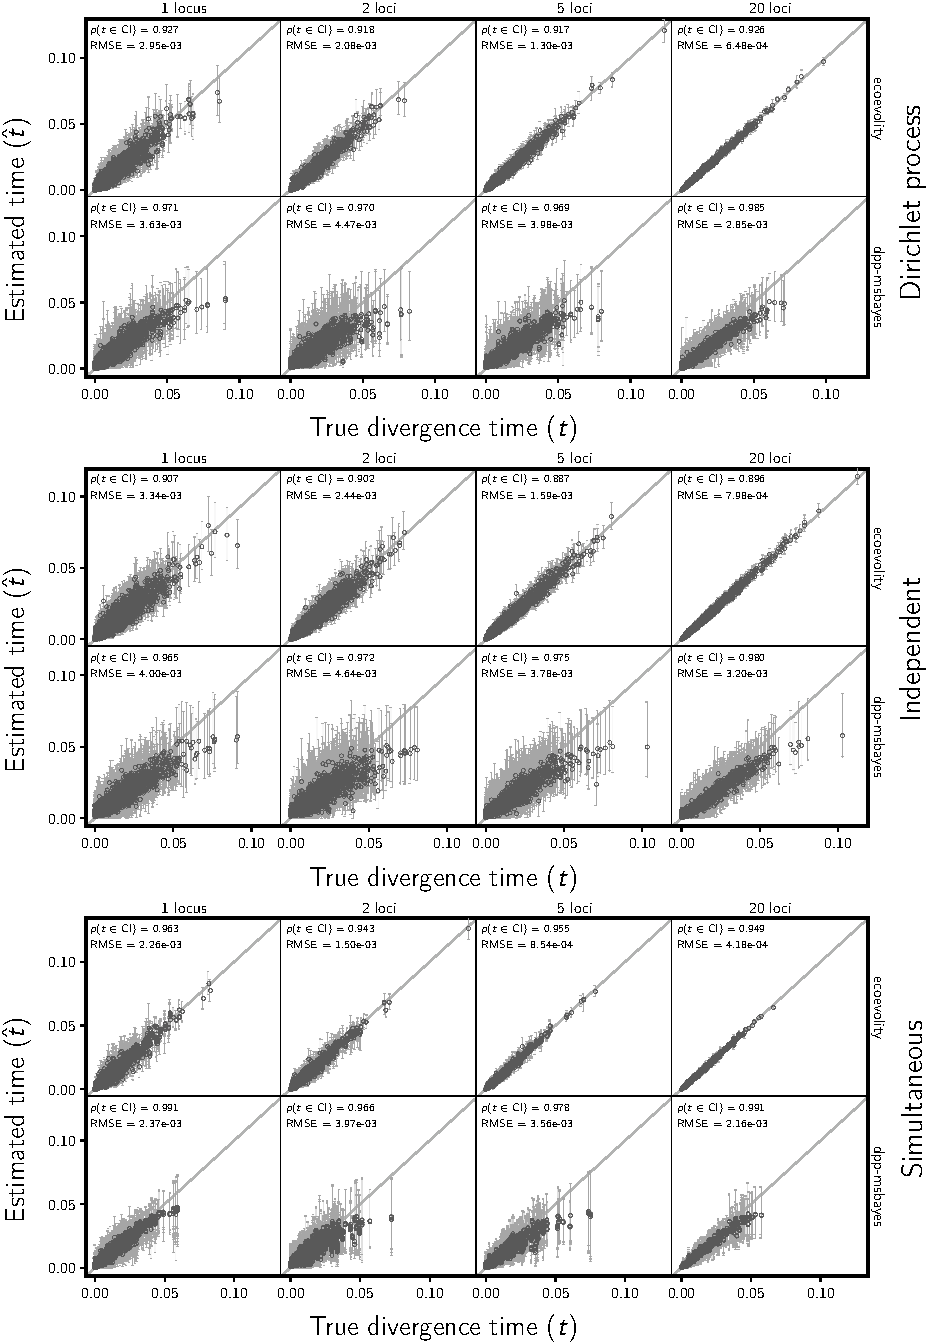
\includegraphics[width=\textwidth,height=0.9\textheight,keepaspectratio]{../images/from-project-repo/plots/tex-plot-grids/grid-div-time-scatter-cropped.pdf}
        \caption{
            \scriptsize
            \Ecoevolity estimates divergence times more accurately
            and precisely than \dppmsbayes across all simulated
            numbers of loci (columns) for five pairs of populations simulated
            to have diverged according to a dirichlet process (top 8 plots),
            independently (middle 8 plots),
            or simultaneously (bottom 8 plots).
            Each plotted circle and associated error bars represent the posterior mean
            and 95\% credible interval.
            \accuracyscatterplotannotations{\comparisonetime{}}
        }
        \label{fig:divtimescatter}
    \end{center}
\end{figure}

\clearpage

\begin{figure}[htbp]
    \begin{center}
        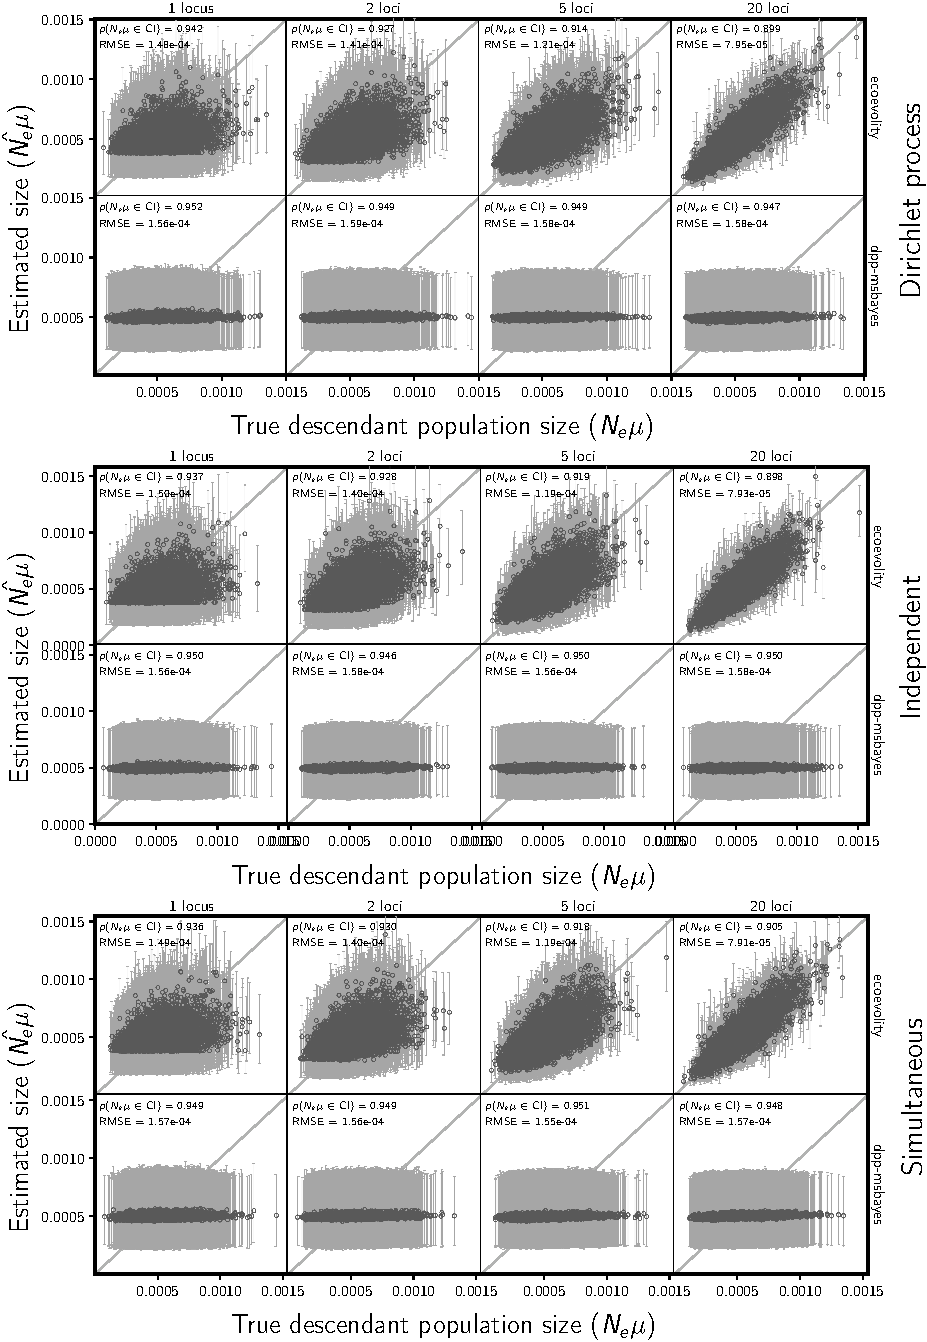
\includegraphics[width=\textwidth,height=0.9\textheight,keepaspectratio]{../images/from-project-repo/plots/tex-plot-grids/grid-leaf-pop-size-scatter-cropped.pdf}
        \caption{
            \scriptsize
            \Ecoevolity estimates the effective sizes of the
            descendant populations more accurately and precisely than
            \dppmsbayes across all simulated numbers of loci
            (columns) for five pairs of populations simulated to have diverged
            according to a Dirichlet process (top 8 plots),
            independently (middle 8 plots),
            or simultaneously (bottom 8 plots).
            Each plotted circle and associated error bars represent the posterior mean
            and 95\% credible interval.
            \accuracyscatterplotannotations{\epopsize{}}
        }
        \label{fig:leafpopsizescatter}
    \end{center}
\end{figure}

\clearpage

\begin{figure}[htbp]
    \begin{center}
        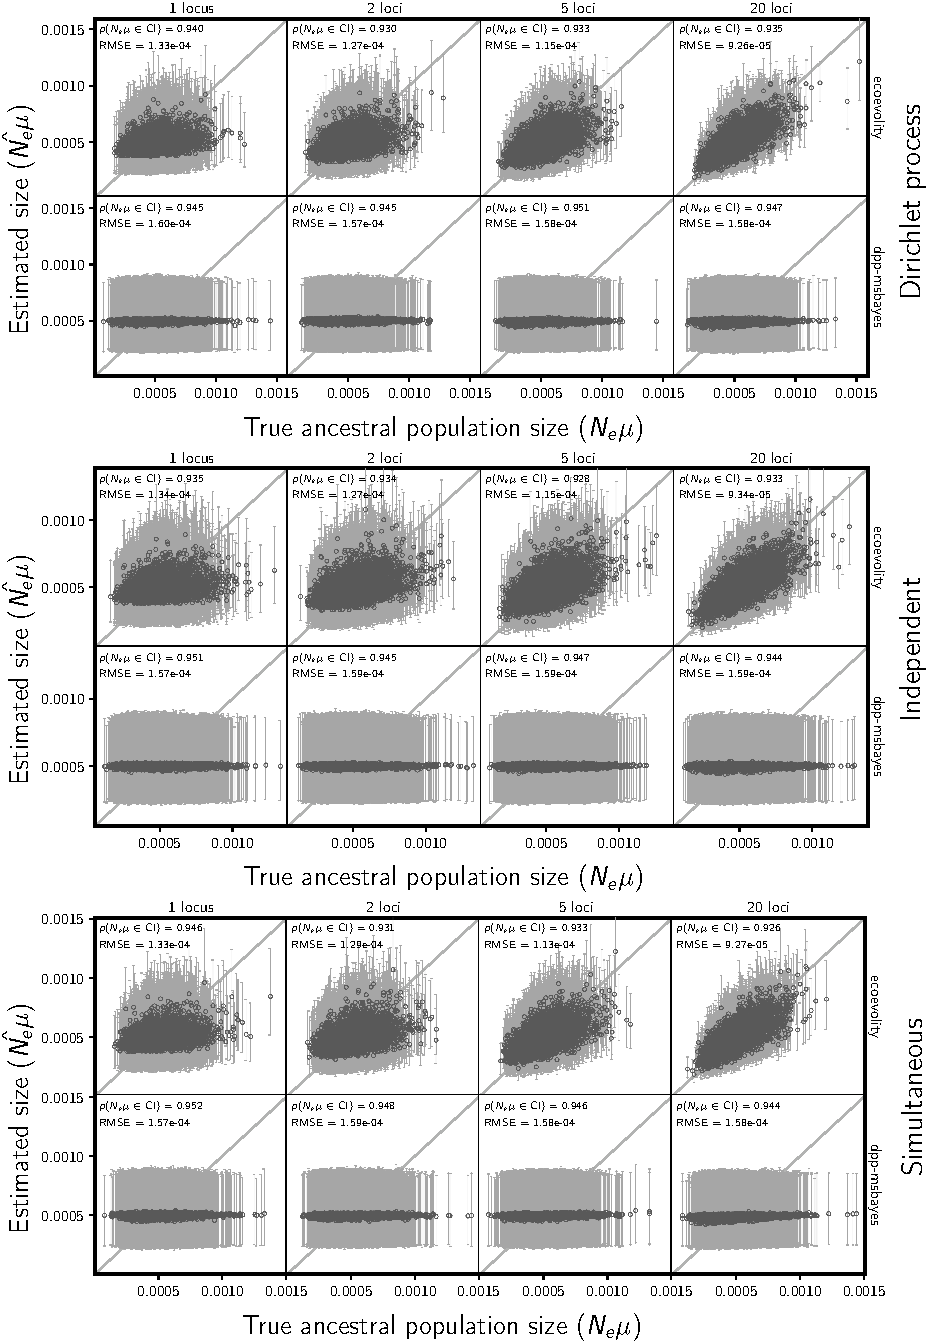
\includegraphics[width=\textwidth,height=0.9\textheight,keepaspectratio]{../images/from-project-repo/plots/tex-plot-grids/grid-root-pop-size-scatter-cropped.pdf}
        \caption{
            \Ecoevolity estimates the effective sizes of the
            ancestral populations more accurately and precisely than
            \dppmsbayes across all simulated numbers of loci
            (columns) for five pairs of populations simulated to have diverged
            according to a Dirichlet process (top 8 plots),
            independently (middle 8 plots),
            or simultaneously (bottom 8 plots).
            Each plotted circle and associated error bars represent the posterior mean
            and 95\% credible interval.
            \accuracyscatterplotannotations{\epopsize{}}
        }
        \label{fig:rootpopsizescatter}
    \end{center}
\end{figure}

\begin{figure}[htbp]
    \begin{center}
        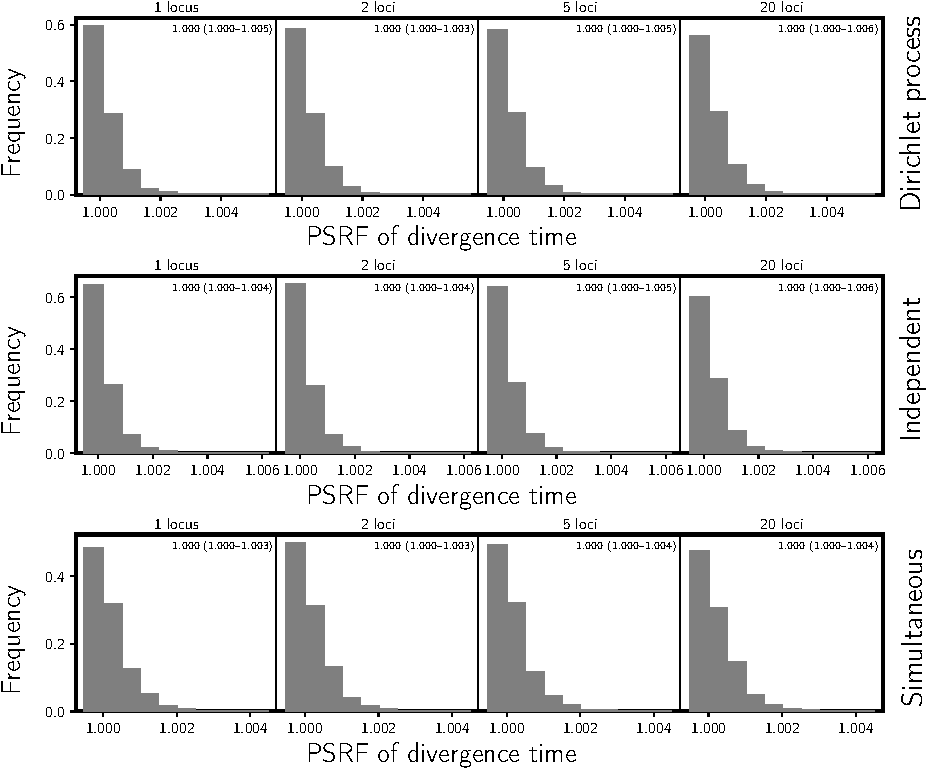
\includegraphics[width=\textwidth,height=0.9\textheight,keepaspectratio]{../images/from-project-repo/plots/tex-plot-grids/grid-psrf-div-time-histograms-cropped.pdf}
        \caption{
            The potential scale reduction factor \citep[PSRF; the square root
            of Equation 1.1 in][]{Brooks1998}
            for the divergence time parameter calculated from the last 1000
            samples of the four MCMC chains run for each simulation replicate.
            The mean PSRF across the 1000 simulation replicates is shown at the
            top right of each plot, followed by the range in parentheses.
        }
        \label{fig:psrfdivtime}
    \end{center}
\end{figure}

\begin{figure}[htbp]
    \begin{center}
        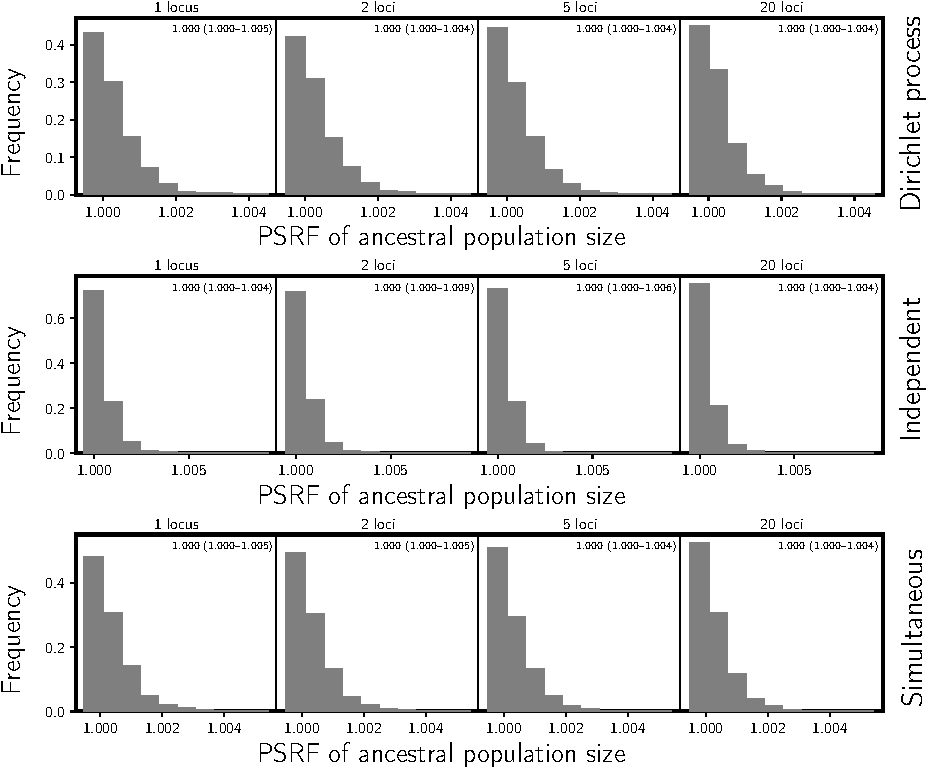
\includegraphics[width=\textwidth,height=0.9\textheight,keepaspectratio]{../images/from-project-repo/plots/tex-plot-grids/grid-psrf-root-pop-size-histograms-cropped.pdf}
        \caption{
            The potential scale reduction factor \citep[PSRF; the square root
            of Equation 1.1 in][]{Brooks1998}
            for the ancestral population size calculated from the last 1000
            samples of the four MCMC chains run for each simulation replicate.
            The mean PSRF across the 1000 simulation replicates is shown at the
            top right of each plot, followed by the range in parentheses.
        }
        \label{fig:psrfrootpopsize}
    \end{center}
\end{figure}

\begin{figure}[htbp]
    \begin{center}
        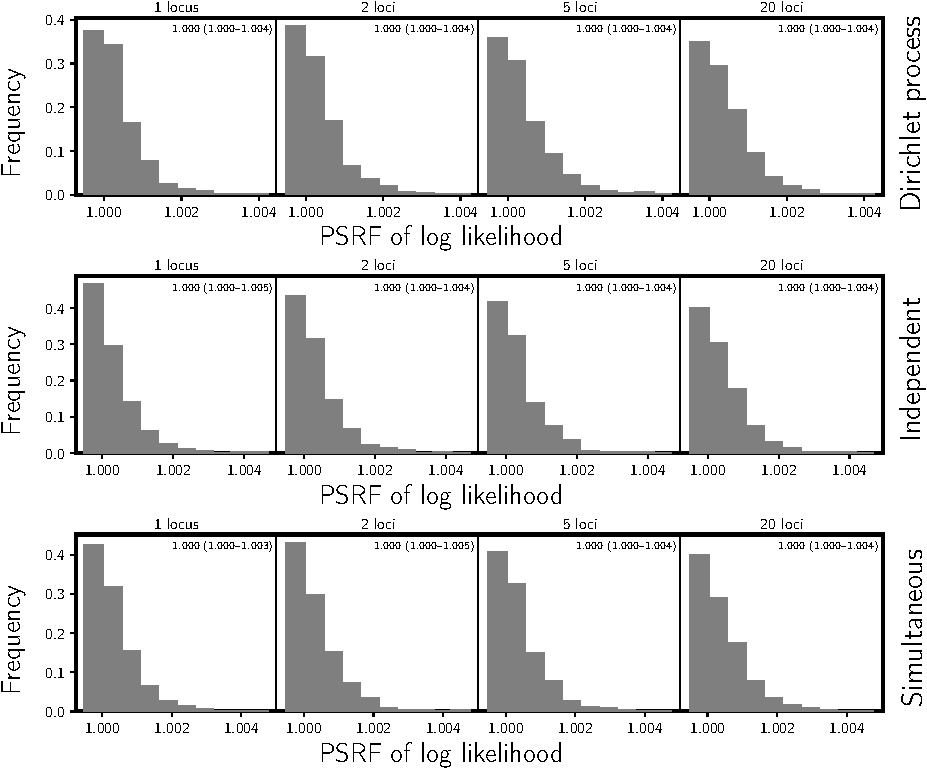
\includegraphics[width=\textwidth,height=0.9\textheight,keepaspectratio]{../images/from-project-repo/plots/tex-plot-grids/grid-psrf-lnl-histograms-cropped.pdf}
        \caption{
            The potential scale reduction factor \citep[PSRF; the square root
            of Equation 1.1 in][]{Brooks1998}
            for the log likelihood calculated from the last 1000
            samples of the four MCMC chains run for each simulation replicate.
            The mean PSRF across the 1000 simulation replicates is shown at the
            top right of each plot, followed by the range in parentheses.
        }
        \label{fig:psrflnl}
    \end{center}
\end{figure}

\begin{figure}[htbp]
    \begin{center}
        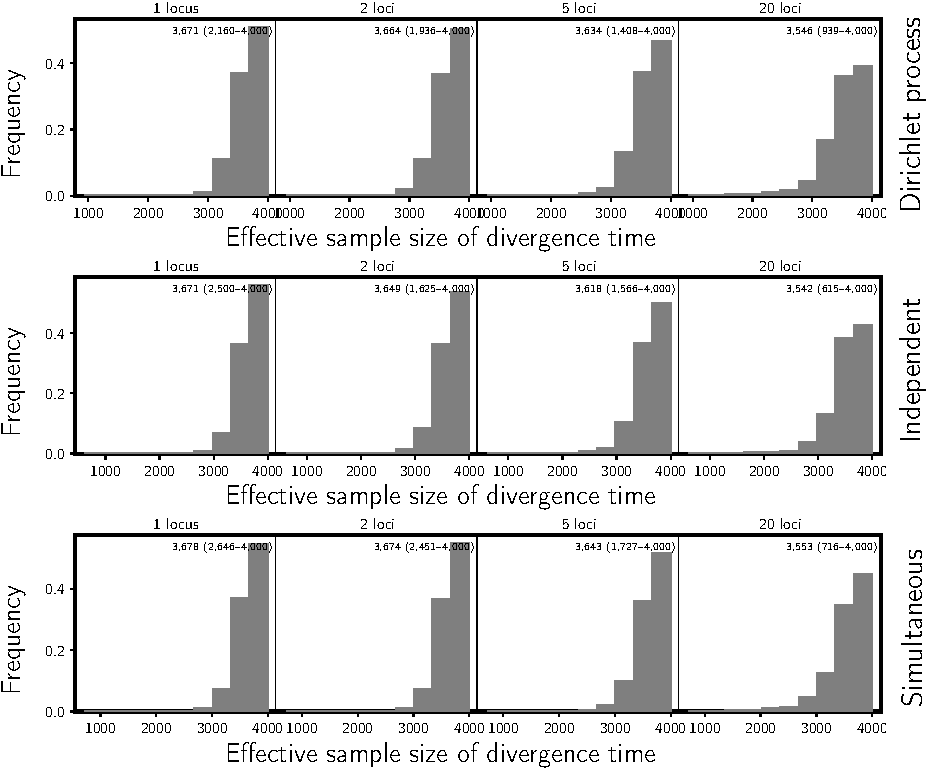
\includegraphics[width=\textwidth,height=0.9\textheight,keepaspectratio]{../images/from-project-repo/plots/tex-plot-grids/grid-ess-div-time-histograms-cropped.pdf}
        \caption{
            The effective sample size \citep[ESS;][]{Gong2014} for the
            divergence time parameter calculated from the last 1000 samples of
            the four MCMC chains run for each simulation replicate.
            The mean ESS across the 1000 simulation replicates is shown at the
            top right of each plot, followed by the range in parentheses.
        }
        \label{fig:essdivtime}
    \end{center}
\end{figure}

\begin{figure}[htbp]
    \begin{center}
        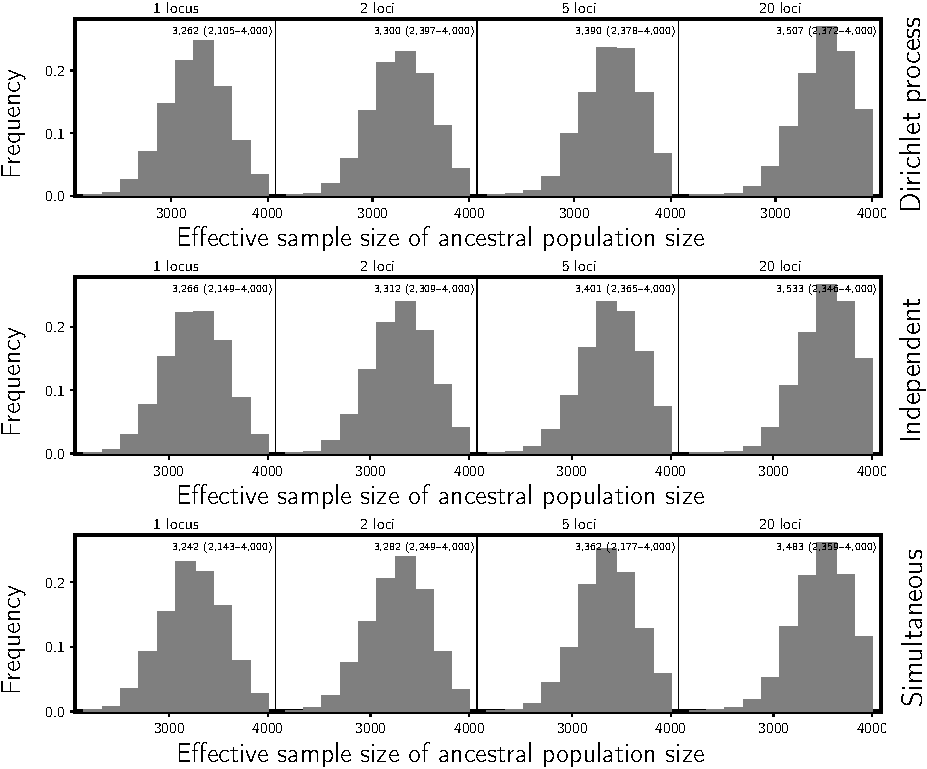
\includegraphics[width=\textwidth,height=0.9\textheight,keepaspectratio]{../images/from-project-repo/plots/tex-plot-grids/grid-ess-root-pop-size-histograms-cropped.pdf}
        \caption{
            The effective sample size \citep[ESS;][]{Gong2014} for the
            ancestral population size calculated from the last 1000 samples of
            the four MCMC chains run for each simulation replicate.
            The mean ESS across the 1000 simulation replicates is shown at the
            top right of each plot, followed by the range in parentheses.
        }
        \label{fig:essrootpopsize}
    \end{center}
\end{figure}

\begin{figure}[htbp]
    \begin{center}
        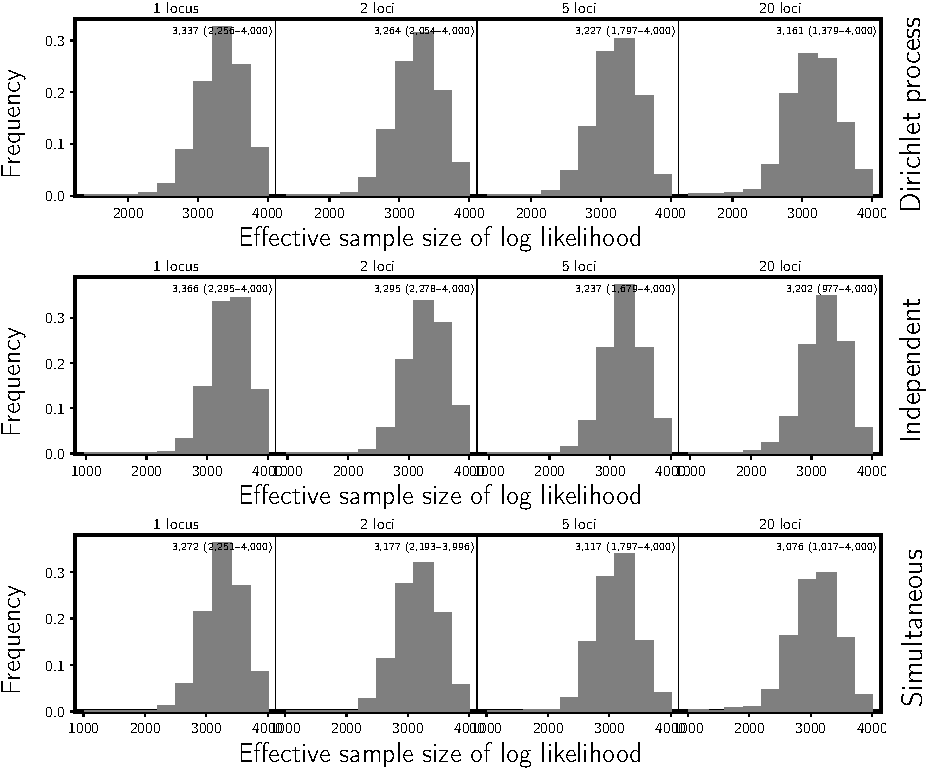
\includegraphics[width=\textwidth,height=0.9\textheight,keepaspectratio]{../images/from-project-repo/plots/tex-plot-grids/grid-ess-lnl-histograms-cropped.pdf}
        \caption{
            The effective sample size \citep[ESS;][]{Gong2014} for the
            log likelihood calculated from the last 1000 samples of
            the four MCMC chains run for each simulation replicate.
            The mean ESS across the 1000 simulation replicates is shown at the
            top right of each plot, followed by the range in parentheses.
        }
        \label{fig:esslnl}
    \end{center}
\end{figure}
